\documentclass[12pt]{article}
\usepackage{amsmath}
\usepackage{amssymb}
\usepackage{geometry}
\usepackage{enumerate}
\usepackage{natbib}
\usepackage{float}%稳定图片位置
\usepackage{graphicx}%画图
\usepackage[english]{babel}
\usepackage{a4wide}
\usepackage{indentfirst}%缩进
\usepackage{enumerate}%加序号
\usepackage{multirow}%合并行
\title{\large UM-SJTU JOINT INSTITUTE\\Data Structures and Algorithms\\(VP281)\\\ \\\ \\\ \\\ \\\ \\\ \\\ \\\ \\\ \\\ \\\
Programming Assignment\\\ \\\ Programming Assignment Two\\\  Linear-Time Selection \\\ \\\ \\\ \\\ \\\ }
\author{Name: Pan Chongdan\\ID: 516370910121}
\date{Date: \today}

\begin{document}
\maketitle
\newpage
\section{Introduction}
The programming assignment asks me to implement two linear time selection algorithms including random selection and deterministic algorithm. The goal is clear, to gain experience in implementing these two sorting algorithms to find the n-th small number in a given random array. 
\par Second, the assignment asks me to study the performance of these 2 studies by studying their time efficiency. In lecture slides 5, professor gives a summary for the time required to complete the selection.
\begin{figure}[H]
\centering
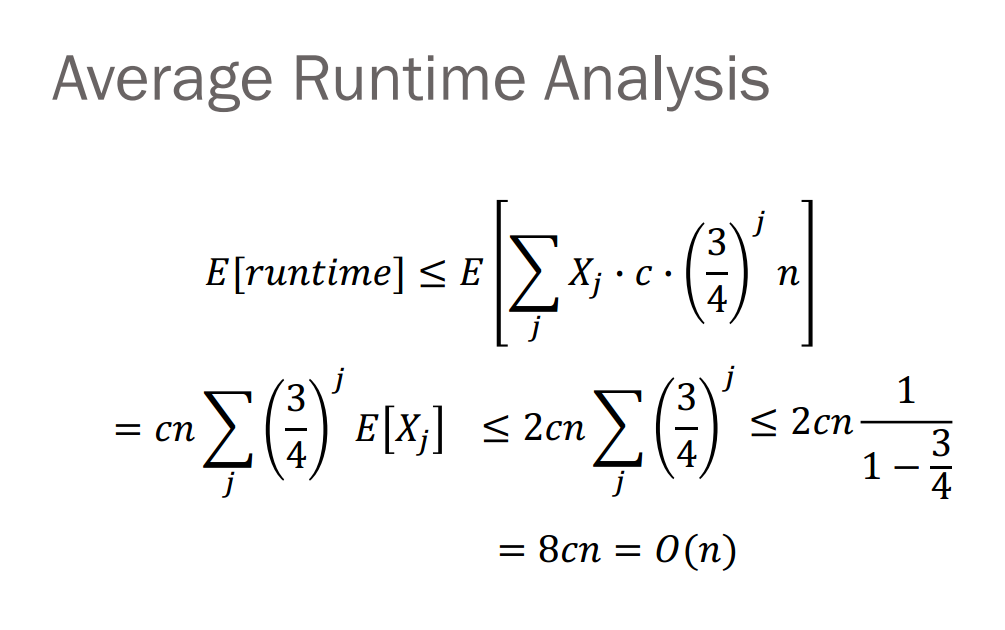
\includegraphics[scale=0.2]{P1.png}
\caption{Random Selection}
\end{figure}
\begin{figure}[H]
\centering
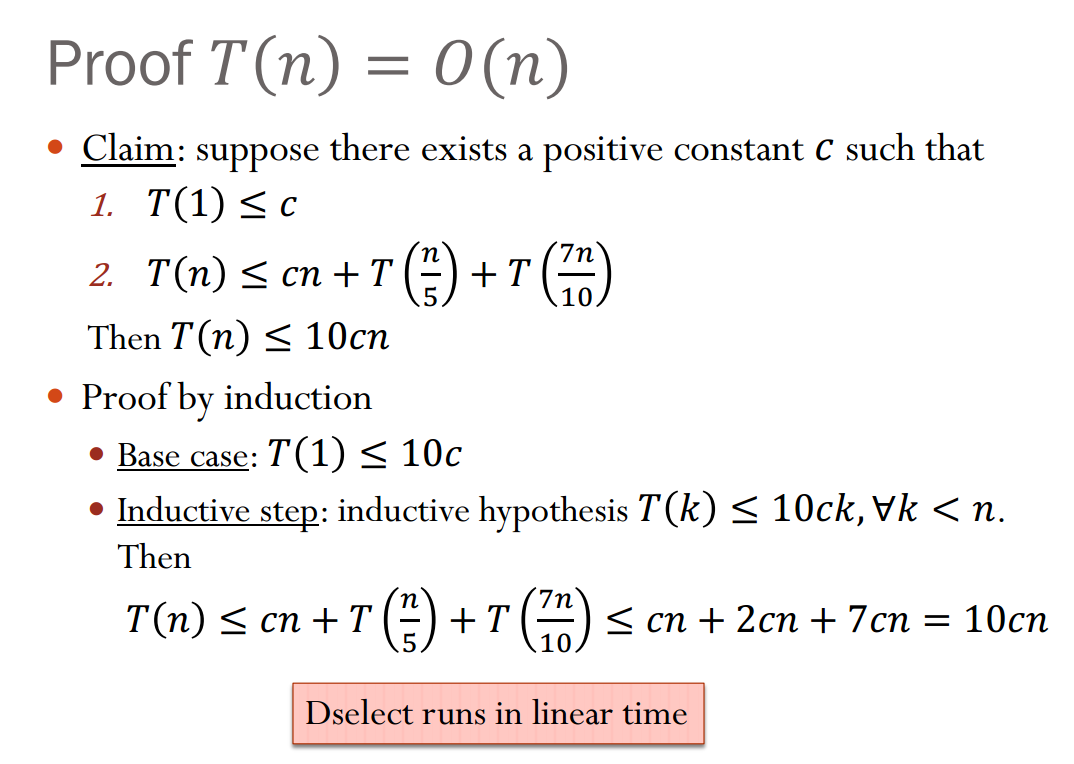
\includegraphics[scale=0.2]{P2.png}
\caption{Deterministic Selection}
\end{figure}
\par However, we need to test the algorithms' time efficiency by ourselves, so I wrote a cpp file to print out the time required for each algorithm, which is included in appendix part.
\section{Result}
To test time efficiency, I used clock() function to get the time required. To get rid of other disturbing factor, I used to variable start and stop to get the time right before and after the sorting complete, then their difference is the time used. In my analysis, I get 10 set of data ,from which the sorted array' size is 100, 500, 1000, 5000, 10000, 50000, 100000, 1000000.
\begin{table}[H]
\centering
\begin{tabular}{|c|c|c|c|c|c|c|c|c|c|}
\hline
Data Size                 & 100    & 500   & 1000     & 5000    & 10000    & 50000   & 100000   & 1000000  \\ \hline
Random Selection               &8e-6& 2.5e-5& 4e-5 & 2.5e-4 & 4e-4 & 4.6e-3 & 7.5e-3 &5.2e-2      \\ \hline
Deterministic Selection        &1.4e-5& 6.4e-4& 8.6e-4 & 6e-4 & 4.4e-4 & 1.7e-3 & 3.3e-3 &3.3e-1  \\ \hline
Quick Sort (in place)     &1.8e-5& 1.2e-4 & 2.1e-4 & 4.1e-4 & 9.6e-4 & 4.0e-3& 8.3e-3 & 9e-2  \\ \hline
\end{tabular}
\end{table}
\section{Conclusion}
This chart is plot by matlab, showing the time efficiency of each algorithms compared to each other, and it has following characteristics.
\begin{figure}[H]
\centering
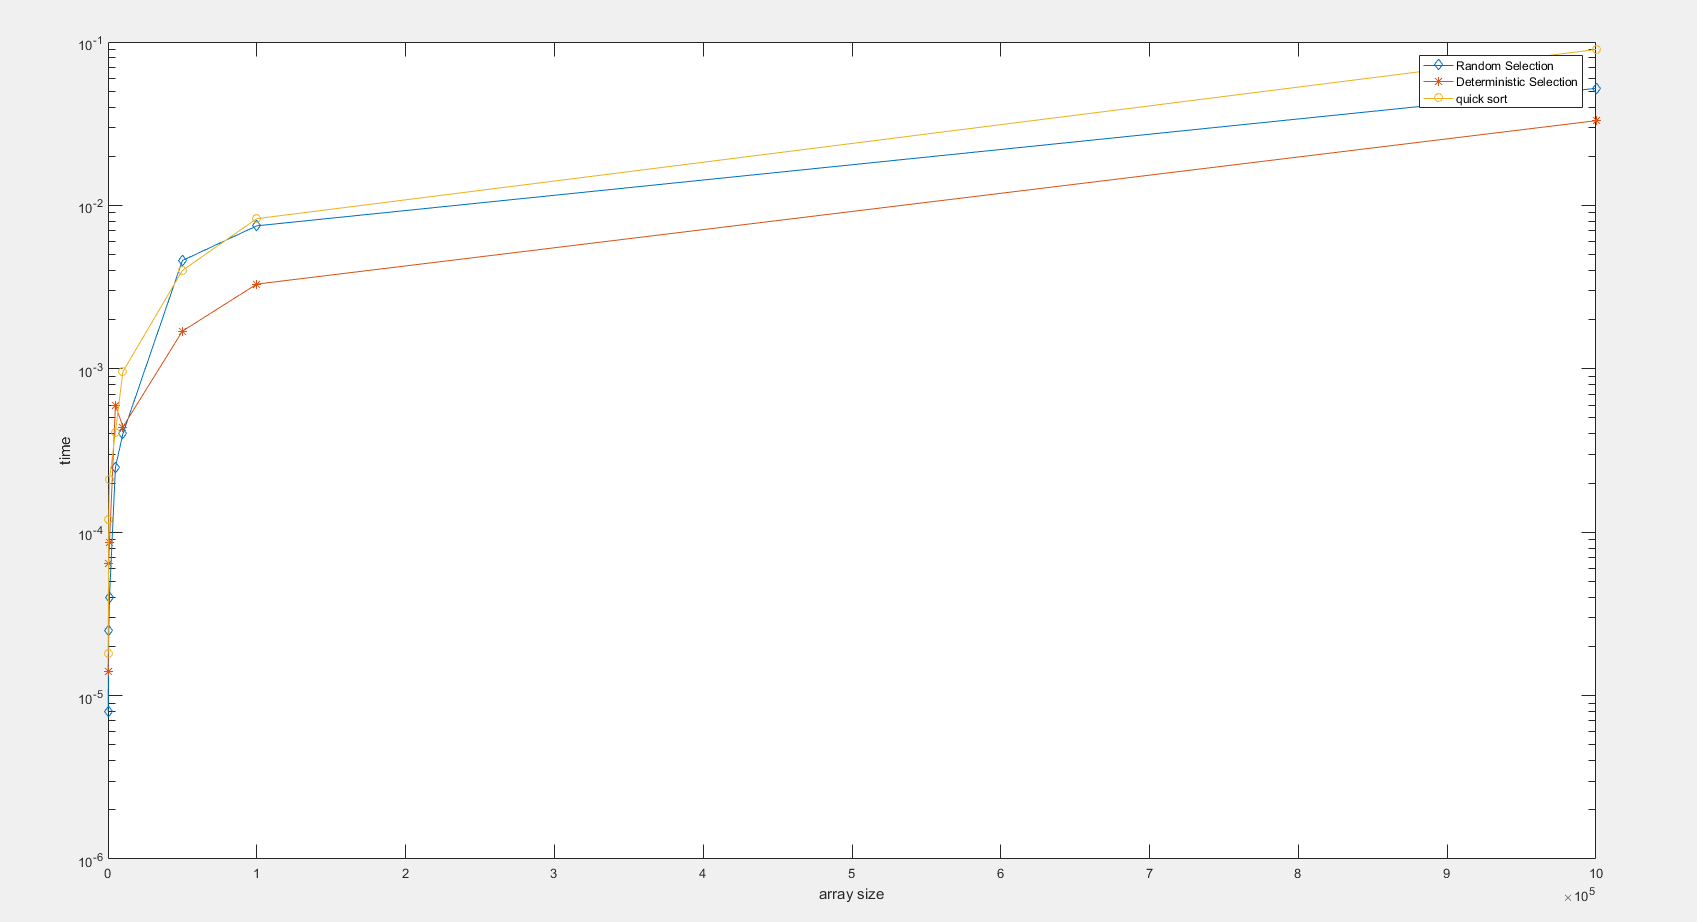
\includegraphics[scale=0.2]{P3.png}
\end{figure}
\begin{enumerate}
\item The average time required for each algorithm grows as the array grows bigger.
\item These three algorithm runs in a linear time when the array is big
\item As shown in the graph and lecture slides, deterministic selection requires the more time than the random selection and they're all quicker than quick sort when the array is big. Also these three ways are all Big O complexity.
\end{enumerate}
\section{Appendix}
The appendix shows the cpp code for main project and time comparison.
\begin{figure}[H]
\centering
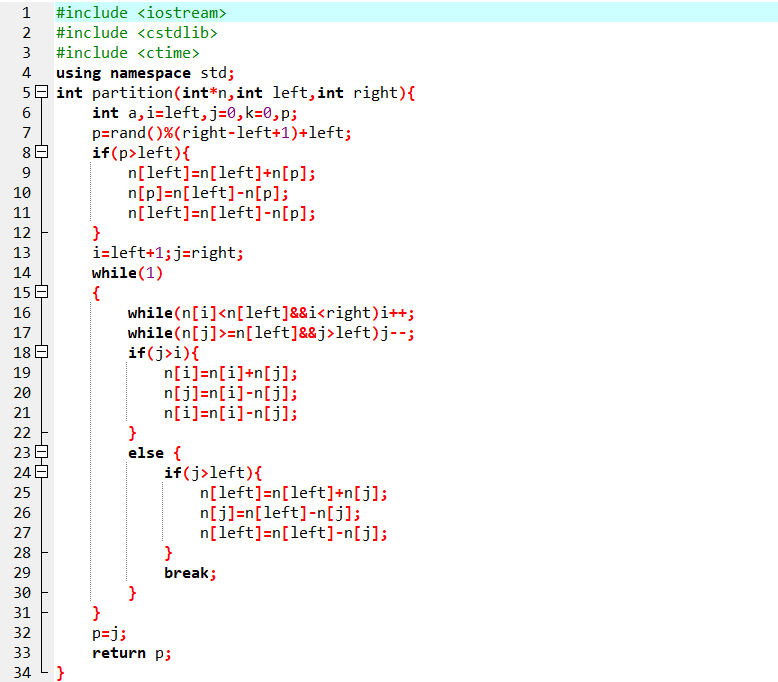
\includegraphics[scale=0.6]{P4.png}
\end{figure}
\begin{figure}[H]
\centering
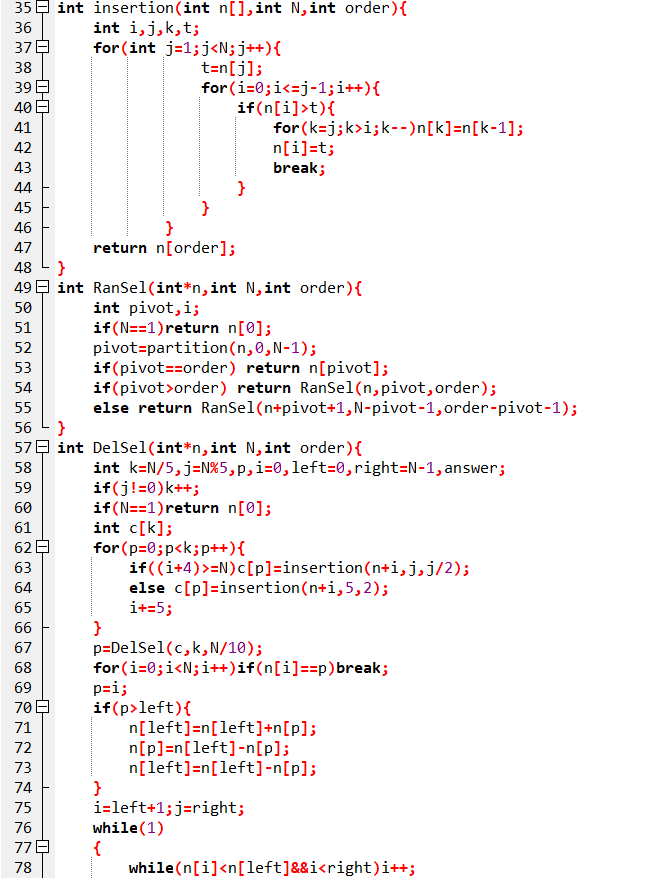
\includegraphics[scale=0.6]{P5.png}
\end{figure}
\begin{figure}[H]
\centering
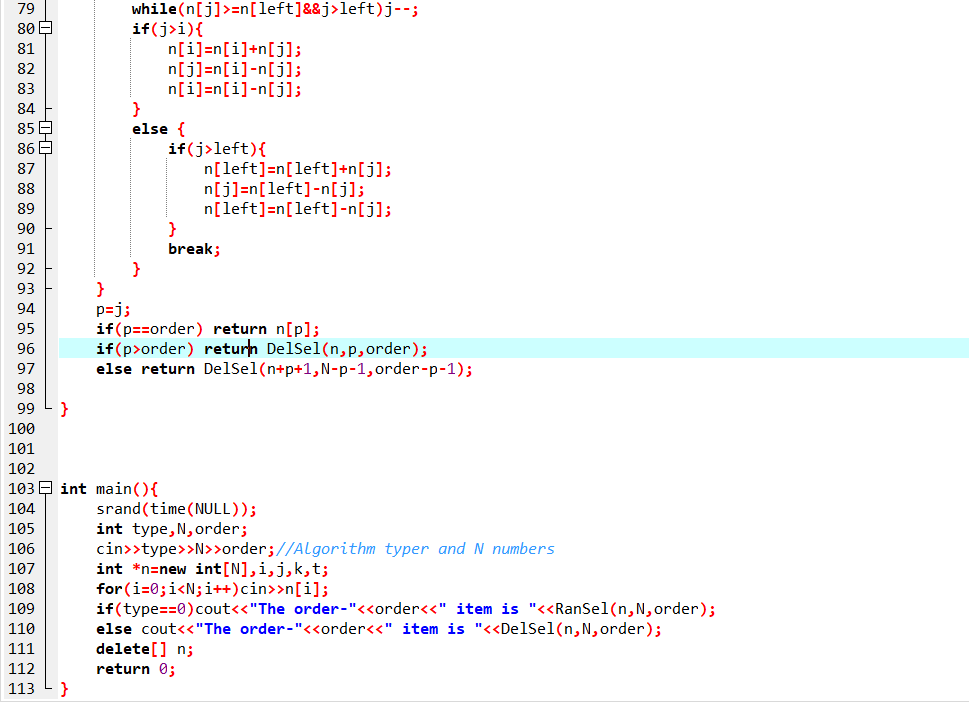
\includegraphics[scale=0.6]{P6.png}
\end{figure}
Then the appendix shows the cpp code for each sort algorithm
\begin{figure}[H]
\centering
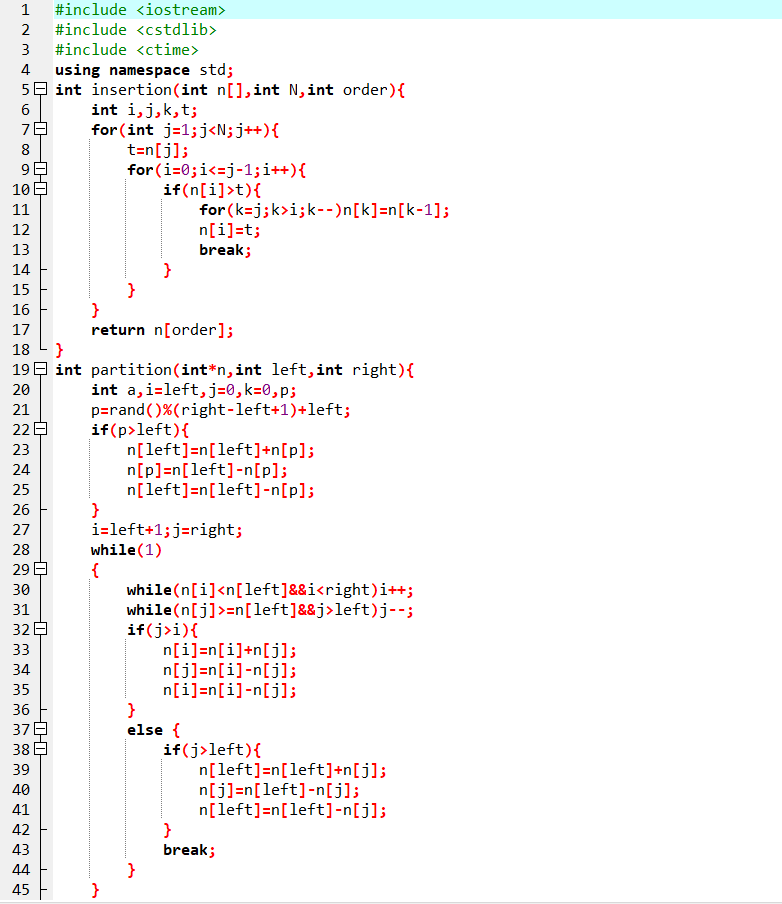
\includegraphics[scale=0.6]{P7.png}
\end{figure}
\begin{figure}[H]
\centering
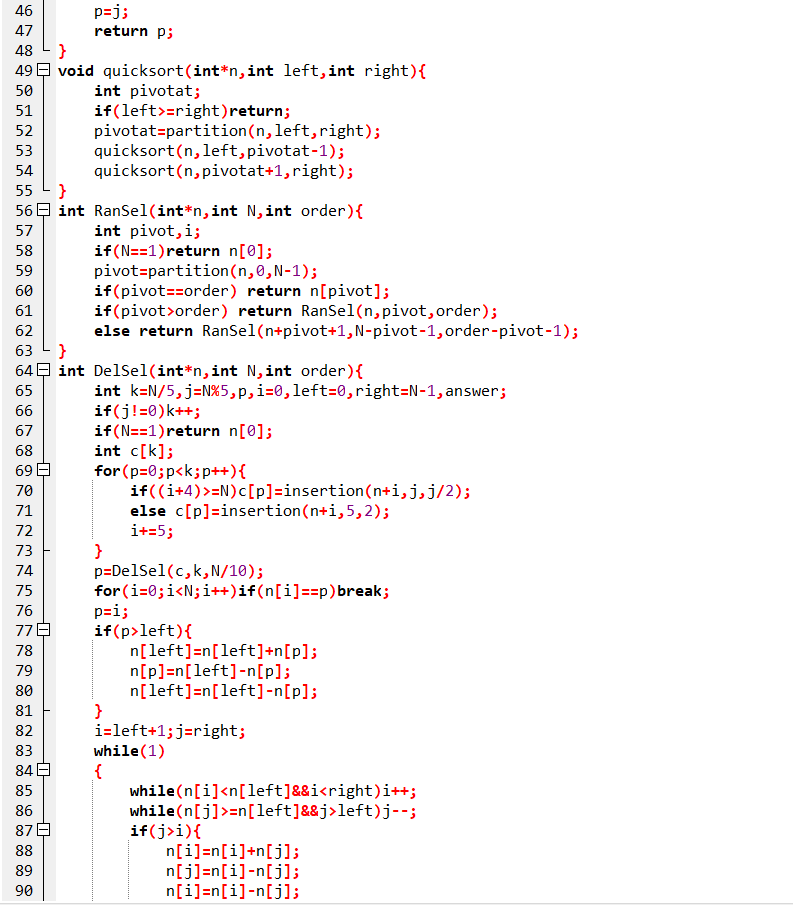
\includegraphics[scale=0.6]{P8.png}
\end{figure}
\begin{figure}[H]
\centering
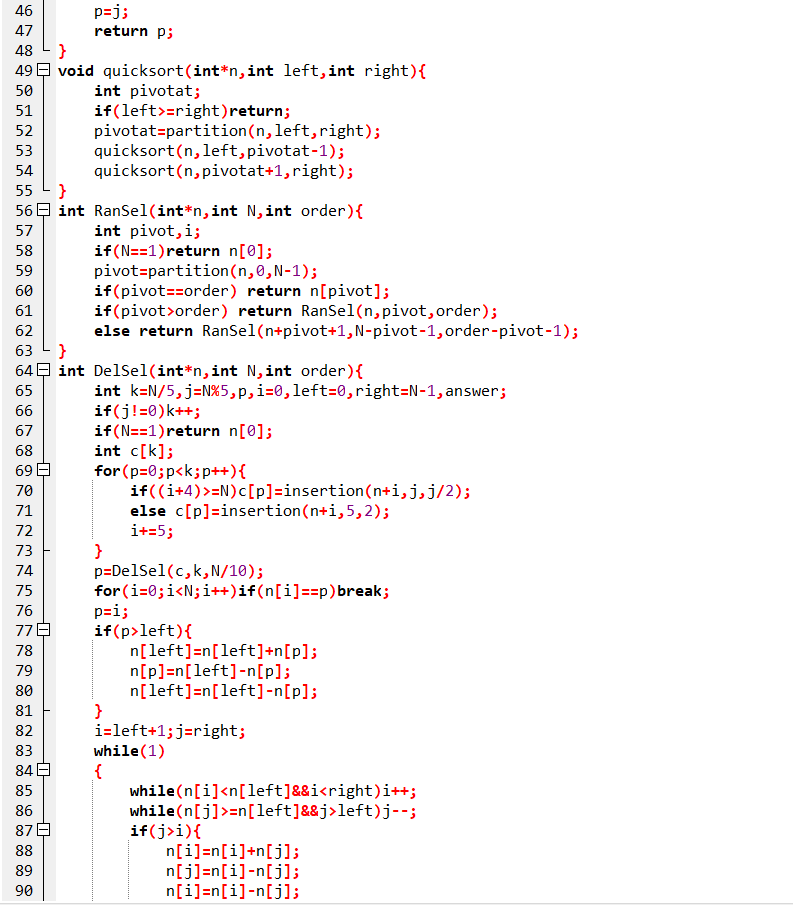
\includegraphics[scale=0.6]{P8.png}
\end{figure}
\begin{figure}[H]
\centering
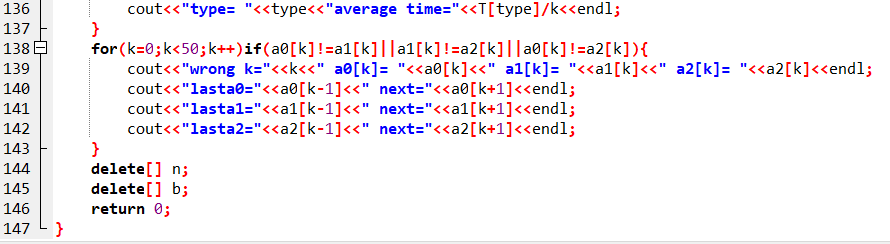
\includegraphics[scale=0.6]{P10.png}
\end{figure}
\end{document}